\section{Transistor come emitter follower}

Per assemblare i seguenti circuiti, non avendo più bisogno della decade di resistenze e del LED, abbiamo deciso di smontare il circuito precedente e ricominciare \emph{ex novo}.

\begin{wrapfigure}[16]{r}[0pt]{36mm}
	\caption{cc3}
	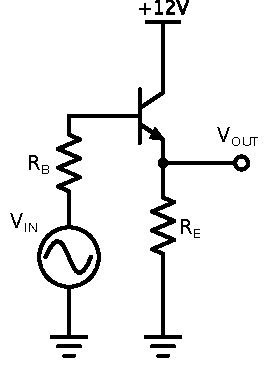
\includegraphics[height=45mm]{cc3.pdf}
	\label{fig:cc3}
\end{wrapfigure}

\subsection{emitter follower}
Il nuovo circuito, mostrato in Fig. \ref{fig:cc3}, è stato alimentato tramite il generatore di forme d'onda con un'onda sinusoidale ad una tensione picco-picco $V_{pp} = \SI{10}{\volt}$.
Il valori delle reistenze erano $R_E = \SI{4655.0}{\ohm}$ e $R_B = \SI{2002.4}{\ohm}$.
Per osservare il segnale in uscita è stato collegato l'oscilloscopio all'emettitore del transistor.

Una volta collegato il circuito, abbiamo osservato che variando la frequenza tra \SI{1}{\kilo\hertz} e \SI{20}{\kilo\hertz} l'immagine mostrata a schermo dall'oscilloscopio, se escludiamo la scala temporale di riferimento, non variava.
Il segnale in output era infatti sempre in fase con il segnale in input, come si può osserare dall'immagine in Fig. \ref{fig:cc3+cc4}, che rappresenta la situazione per $f = \SI{20}{\kilo\hertz}$.
Inoltre il segnale in output (tratteggiato) è in modulo sempre minore del segnale in input.

$$spiegazione \quad della \quad differenza \quad tra \quad il \quad modulo \quad dei \quad due \quad segnali$$
Infine, in corrispondenza di ogni semionda negativa, in segnale in output era nullo.
Tale fenomeno è chiamato ``\emph{clamping}''.

$$MOTIVAZIONE \qquad taglio \,\, semionda \,\, negativa \quad (clamping)$$
\begin{figure}[h]
\centering
	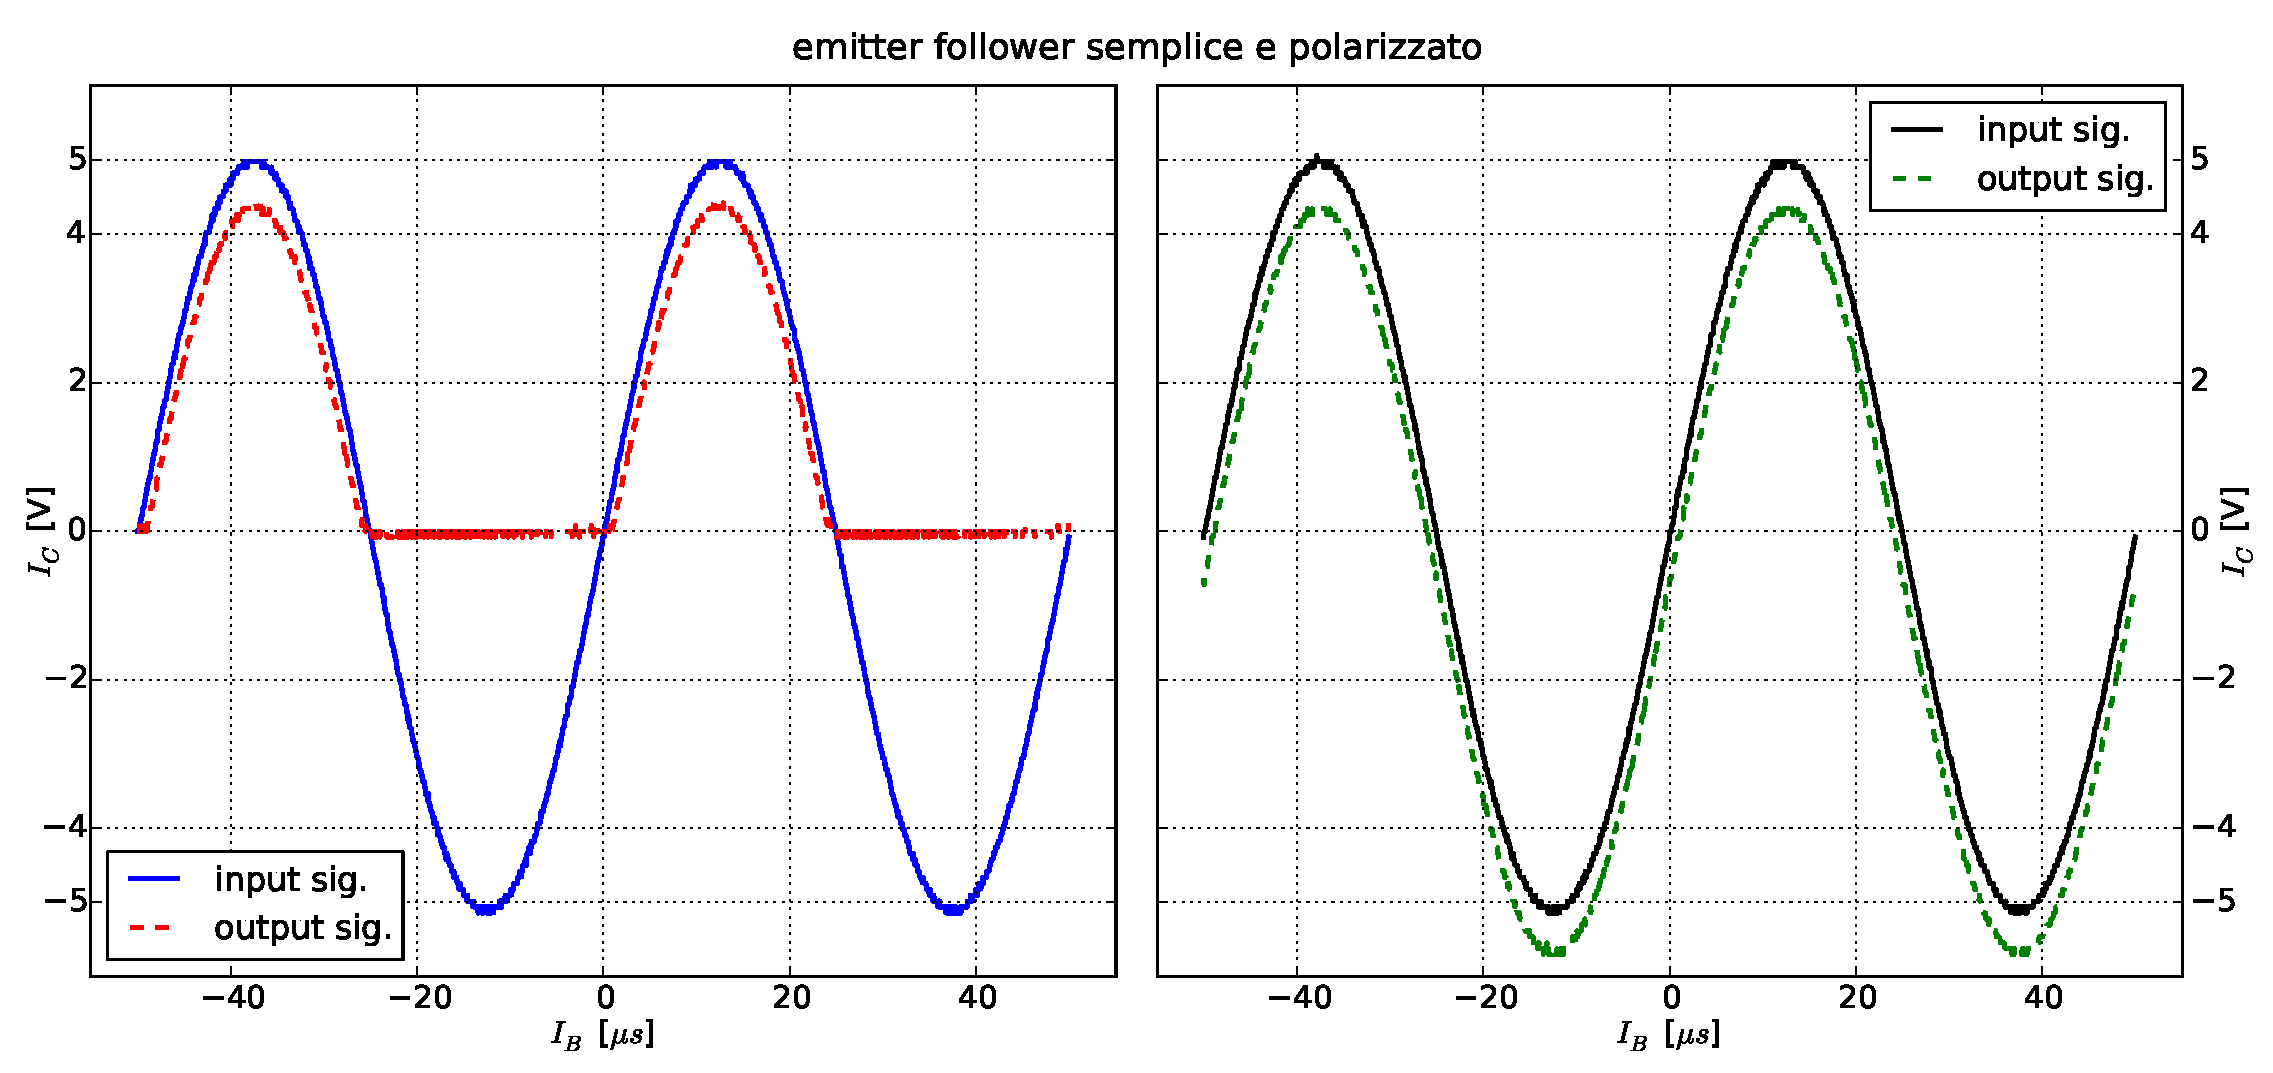
\includegraphics[width=0.85\textwidth]{cc3+cc4.pdf}
	\caption{Nel grafico a sinistra sono rappresentati i segnali in input e in output al circuito del emitter follower semplice, mentre a destra sono rappresentati i segnali dell'emitter follower polarizzato. Entrambi i segnali sono stati ricavati con una frequenza di $V_{in}$ di \SI{20}{\kilo\hertz}.}
	\label{fig:cc3+cc4}
\end{figure}

\begin{wrapfigure}[12]{l}[0pt]{36mm}
	\caption{cc4}
	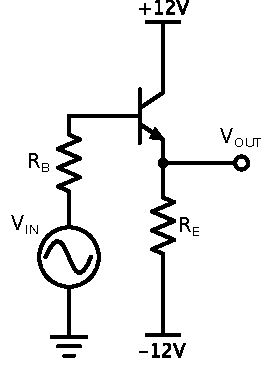
\includegraphics[height=45mm]{cc4.pdf}
	\label{fig:cc4}
\end{wrapfigure}

\subsection{emitter follower polarizzato}
Per polarizzare il transistor, come mostrato dal circuito in Fig. \ref{fig:cc4}, è bastato collegare un capo della resistenza $R_E$ al polo negativo del generatore di corrente continua anziché a massa.
I componenti circuitali sono pertanto rimasti i medesimi del circuito emitter follower ``semplice''.
Questa modifica al circuito è stata fatta per evitare, almeno parzialmente, il fenomeno di ``clamping''.

Anche in questo caso abbiamo variato la frequenza dell'onda quadra nello stesso range preso in considerazione precedentemente: il risultato è mostrato in Fig. \ref{fig:cc3+cc4}.
Ancora una volta il segnale in output è in fase con il segnale in input.
Evitando il fenomeno di ``clamping'', abbiamo ottenuto in output un segnale sinusoidale con la stessa $V_{pp}$ e frequenza di quello in input, però abbassato di circa $\SI{0.6}{\volt}$.

\begin{wrapfigure}[6]{r}[0pt]{36mm}
	\caption{cc5}
	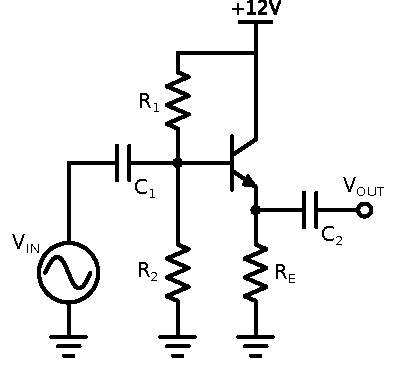
\includegraphics[height=45mm]{cc5.pdf}
	\label{fig:cc5}
\end{wrapfigure}

\subsection{emitter follower con partitore}
Anche in questo caso, poiché avevamo necessità di aggiungere diversi componenti al circuito, abbiamo staccato tutti i componenti dalla breadboard e assemblato il circuito da zero.

\begin{figure}[h]
\centering
	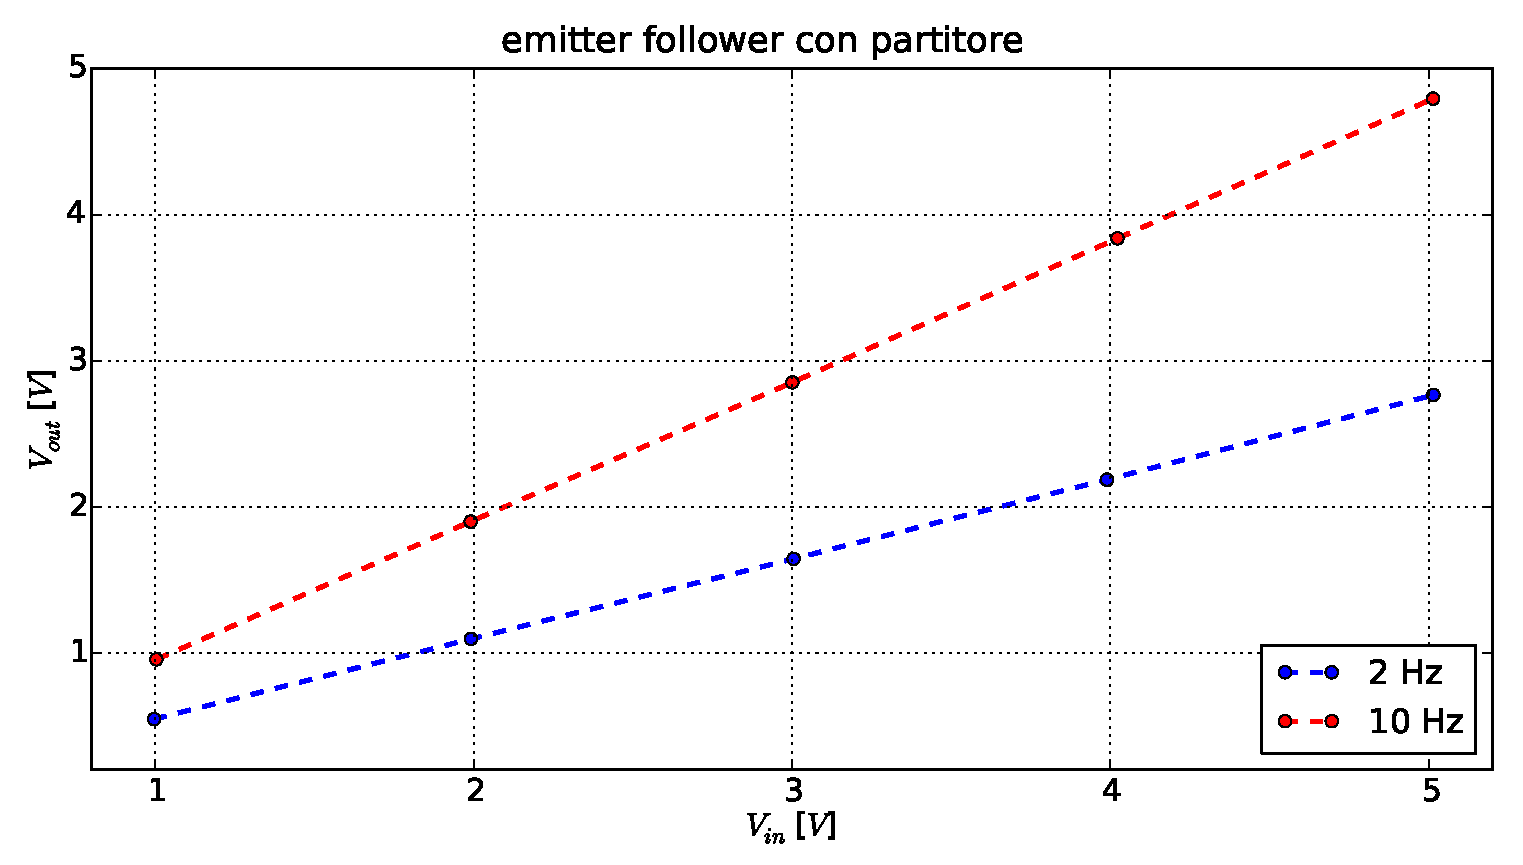
\includegraphics[width=0.7\textwidth]{am.pdf}
	\caption{}
	\label{fig:am}
\end{figure}

\begin{figure}[h]
\centering
	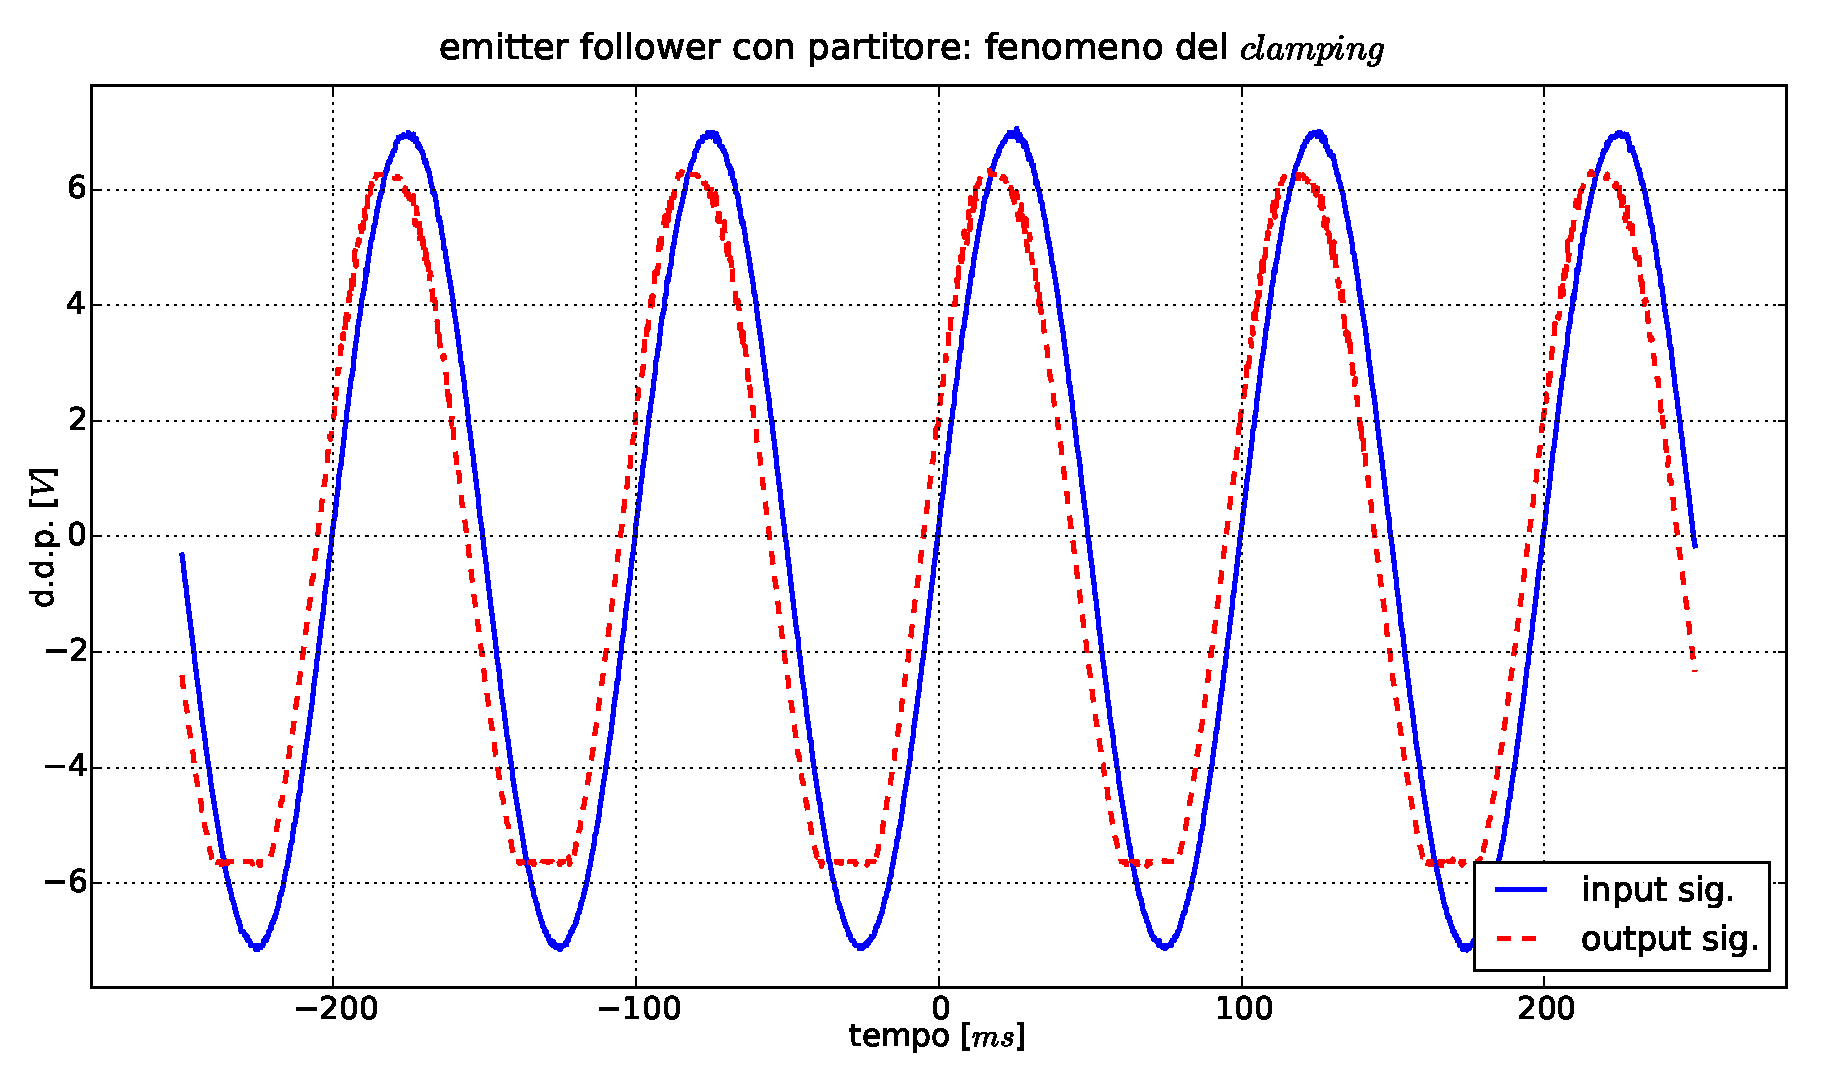
\includegraphics[width=0.7\textwidth]{clamp.pdf}
	\caption{}
	\label{fig:clamp}
\end{figure}

Come già anticipato nella sezione precedente, il fenomeno di ``clamping'' avviene anche nel caso dei circuti emitter follower polarizzato ed emitter follower con partitore.
Ciò succede quando il segnale in ingresso ha un'ampiezza tale da mandare in interdizione (\ref{}) il transistor in tutta o in parte  della semionda negativa.
In Fig. \ref{fig:clamp} è rappresentato il fenomeno nel caso del circuito emitter follower con partitore per i valori di frequenza \SI{122341324}{\hertz} e tensione $V_{pp} = \SI{122341324}{\volt}$